

% \begin{figure}[t]
% 	\centering
% 	\begin{subfigure}[t]{0.3\textwidth}
% 		\centering
% 		\hspace{8mm}
% 		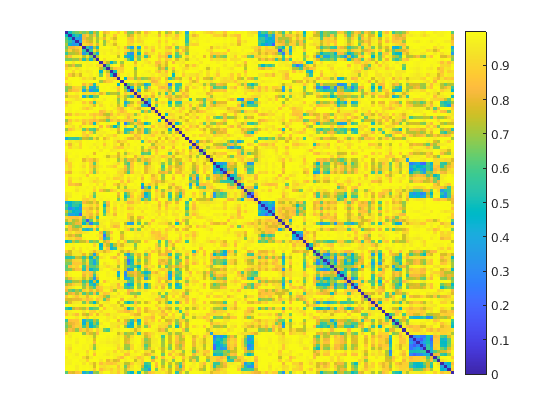
\includegraphics[width=1\textwidth, trim={0cm, 0.0cm, 0.0cm, 0.0cm}]{figures/dfc_645_subject_32_time_68.png}\hfill
% 		\hspace{-15mm}
% 		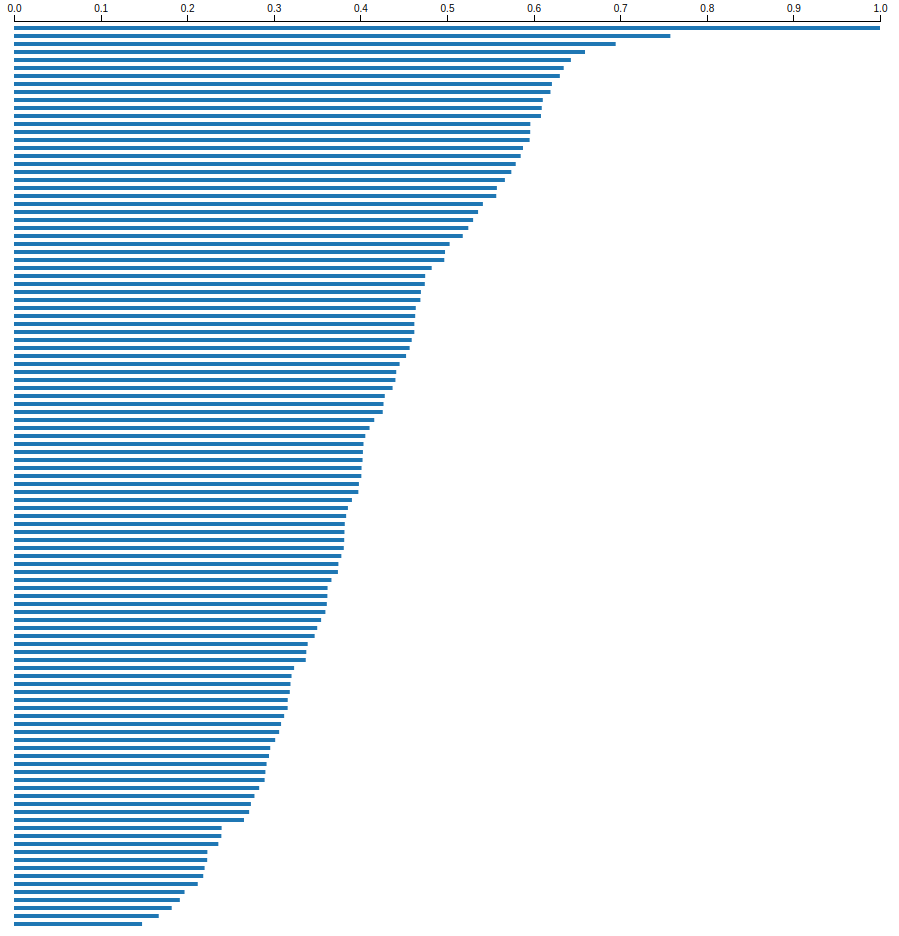
\includegraphics[width=1\textwidth, trim={0cm, 0.0cm, 0.0cm, 0.0cm}, angle=0,origin=a]{figures/dfc_645_subject_32_time_68_barcode.png}
% 		\subcaption{Extracted barcodes of a FCN for $645$ms at $t=68$}
% 	\end{subfigure}
% 	\hfill
% 	\begin{subfigure}[t]{0.3\textwidth}
% 		\centering
% 		\hspace{8mm}
% 		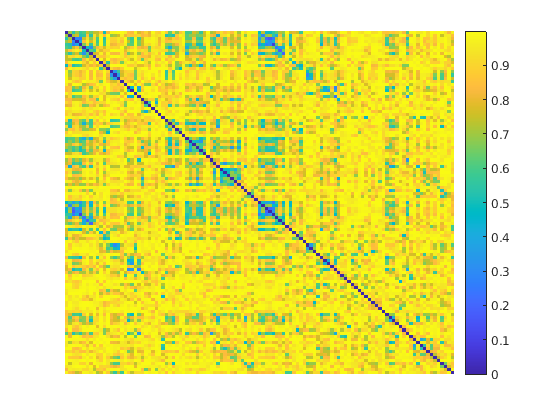
\includegraphics[width=\textwidth, trim={0cm, 0.0cm, 0.0cm, 0.0cm}]{figures/dfc_1400_subject_32_time_68.png}\hfill
% 		\hspace{-15mm}
% 		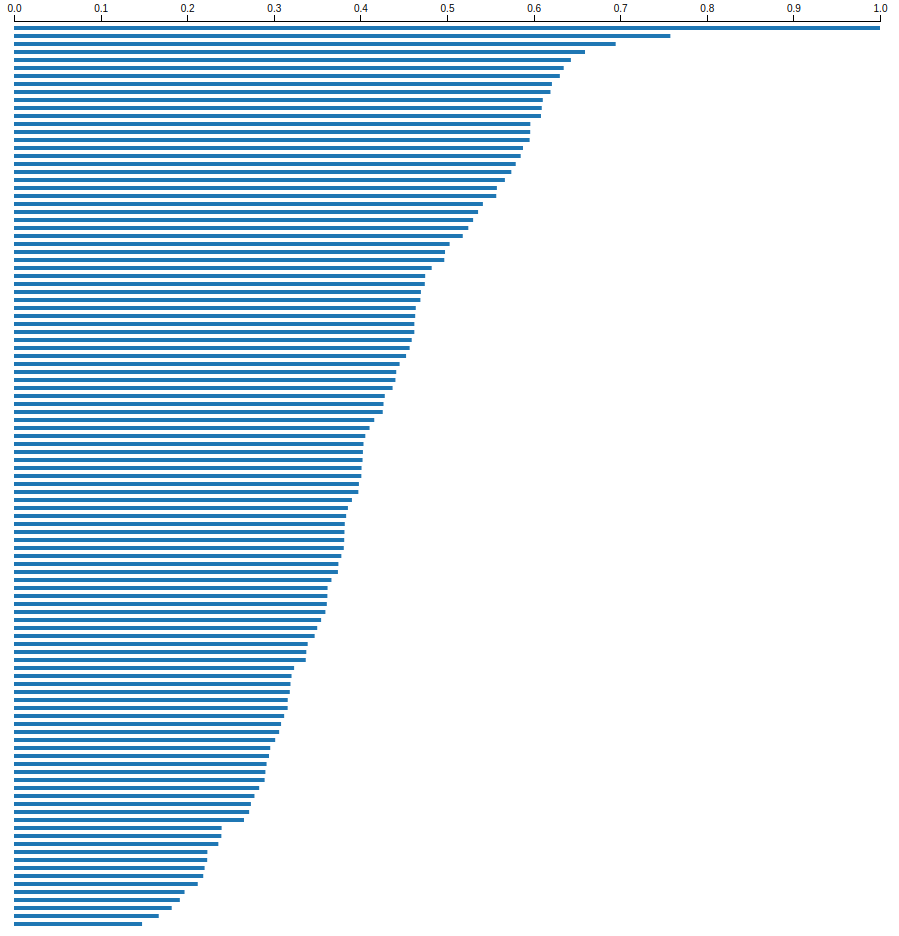
\includegraphics[width=\textwidth, trim={0cm, 0.0cm, 0.0cm, 0.0cm}]{figures/dfc_645_subject_32_time_68_barcode.png}
% 		\subcaption{Extracted barcodes of a FCN for $1400$ms at $t=68$}
% 	\end{subfigure}
% 	\hfill
% 	\begin{subfigure}[t]{0.3\textwidth}
% 		\centering
% 		\hspace{8mm}
% 		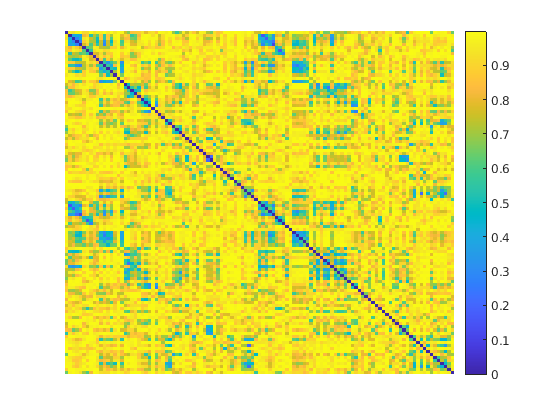
\includegraphics[width=\textwidth, trim={0cm, 0.0cm, 0.0cm, 0.0cm}]{figures/dfc_2500_subject_32_time_68.png}\hfill
% 		\hspace{-15mm}
% 		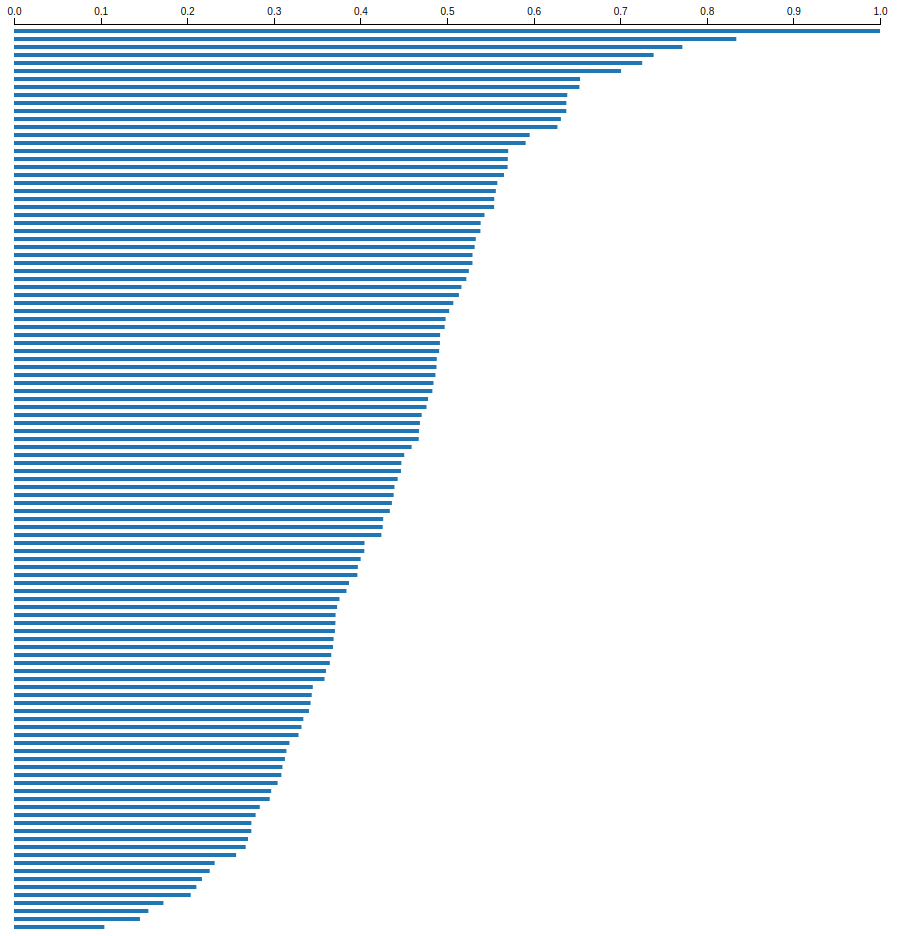
\includegraphics[width=\textwidth, trim={0cm, 0.0cm, 0.0cm, 0.0cm}]{figures/dfc_2500_subject_32_time_68_barcode.png}
% 		\subcaption{Extracted barcodes of a FCN for $2500$ms at $t=68$}
% 	\end{subfigure}
% 	\caption{The FCN (top) and extracted topological feature (bottom) as 0-dimensional barcodes for subject $32$ at $t=68$ for temporal sampling periods $645ms$ (left), $1400ms$ (center), and $2500ms$ (bottom). The matrix size is $113 \times 113$.}
% 	\label{fig:wd1}
% \end{figure}



% \setlength{\tabcolsep}{0.5em} % for the horizontal padding
% {\renewcommand{\arraystretch}{1.2}% for the vertical padding
%     \begin{table}[t]
%         \centering
%         \begin{tabular}
%         {| c | c | c | c | c |}
%          \hline
%             \multirow{2}{*}{Distance} & \multicolumn{2}{c |}{TDA Pipeline} & \multicolumn{2}{c |}{NonTDA Pipeline} \\ \cline{2-5}
%               & Subjects & Percentage & Subjects & Percentage
%              \\ \hline \hline
%              0 & 118 & 37.34\% & 1 & 0.32\% \\ \hline 
%              1 & 70 & 22.15\% & 4 & 1.27\% \\ \hline 
%              2 & 18 & 5.70\% & 9 & 2.85\% \\ \hline 
%              3 & 17 & 5.38\% & 15 & 4.75\% \\ \hline 
%              4 & 22 & 6.96\% & 23 & 7.28\% \\ \hline 
%              5 & 13 & 4.11\% & 35 & 11.08\% \\ \hline 
%              6 & 8 & 2.53\% &  31 & 9.81\% \\ \hline 
%              7 & 11 & 3.48\% & 28 & 8.86\% \\ \hline 
%              8 & 8 & 2.53\% & 34 & 10.76\% \\ \hline 
%              9 & 8 & 2.53\% & 32 & 10.13\% \\ \hline 
%              10 & 6 & 1.90\% & 33 & 10.44\% \\ \hline 
%              11 & 5 & 1.58\% & 32 & 10.13\% \\ \hline 
%              12 & 6 & 1.90\% & 29 & 9.18\% \\ \hline 
%              13 & 6 & 1.90\% & 10 & 3.16\% \\ \hline 
             
%         \end{tabular}
%         \caption{Distance between the number of clusters for the data cohorts for TDA and NonTDA pipeline using Eq. \ref{eq:dis}}
%          \label{tab:clustering}
%     \end{table}   

    % \begin{table}[t]
    %     \label{tab:clustering}
    %     \centering
    %     \begin{tabular}
    %     {| c | c | c | c | c | c | c |}
    %      \hline
    %         \multirow{2}{*}{Distance} & \multicolumn{2}{c |}{TDA} & \multicolumn{2}{c |}{Downsampled TDA} & \multicolumn{2}{c |}{NonTDA} \\ \cline{2-7}
    %           & Subjects & Percentage & Subjects & Percentage & Subjects & Percentage
    %          \\ \hline \hline
    %          0 & 118 & 37.34\% & 158 & 50.00\% & 1 & 0.32\% \\ \hline 
    %          1 & 70 & 22.15\% & 65 & 20.57\% & 4 & 1.27\% \\ \hline 
    %          2 & 18 & 5.70\% & 19 & 6.01\% & 9 & 2.85\% \\ \hline 
    %          3 & 17 & 5.38\% & 8 & 2.53\% & 15 & 4.75\% \\ \hline 
    %          4 & 22 & 6.96\% & 18 & 5.70\% & 23 & 7.28\% \\ \hline 
    %          5 & 13 & 4.11\% & 11 & 3.48\% & 35 & 11.08\% \\ \hline 
    %          6 & 8 & 2.53\% & 4 & 1.27\% & 31 & 9.81\% \\ \hline 
    %          7 & 11 & 3.48\% & 8 & 2.53\% & 28 & 8.86\% \\ \hline 
    %          8 & 8 & 2.53\% & 5 & 1.58\% & 34 & 10.76\% \\ \hline 
    %          9 & 8 & 2.53\% & 4 & 1.27\% & 32 & 10.13\% \\ \hline 
    %          10 & 6 & 1.90\% & 4 & 1.27\% & 33 & 10.44\% \\ \hline 
    %          11 & 5 & 1.58\% &  4 & 1.27\% & 32 & 10.13\% \\ \hline 
    %          12 & 6 & 1.90\% & 6 & 1.90\% & 29 & 9.18\% \\ \hline 
    %          13 & 6 & 1.90\% & 2 & 0.63\% & 10 & 3.16\% \\ \hline 
             
    %     \end{tabular}
    %     \caption{Clustering result for TDA pipeline, downsampled TDA pipeline, and NonTDA pipeline}
    % \end{table}

 
    
%     \begin{table}[t]
%         \centering
%         \begin{tabular}
%         {| c | c | c | c | c | c | c |}
%          \hline
%             \multirow{2}{*}{Distance} & \multicolumn{2}{c |}{$2500ms$ and $1400ms$ } & \multicolumn{2}{c |}{$1400ms$ and $645ms$ } & \multicolumn{2}{c |}{$645ms$ and $2500ms$ } \\ \cline{2-7}
%               & Subjects & Percentage & Subjects & Percentage & Subjects & Percentage
%              \\ \hline \hline
% 0 & 172 & 54.430\% & 176 & 55.696\% & 160 & 50.633\% \\ \hline 
% 1 & 47 & 14.873\% & 61 & 19.304\% & 65 & 20.570\% \\ \hline 
% 2 & 18 & 5.696\% & 12 & 3.797\% & 19 & 6.013\% \\ \hline 
% 3 & 17 & 5.380\% & 11 & 3.481\% & 8 & 2.532\% \\ \hline 
% 4 & 20 & 6.329\% & 9 & 2.848\% & 17 & 5.380\% \\ \hline 
% 5 & 8 & 2.532\% & 9 & 2.848\% & 10 & 3.165\% \\ \hline 
% 6 & 3 & 0.949\% & 8 & 2.532\% & 5 & 1.582\% \\ \hline 
% 7 & 8 & 2.532\% & 6 & 1.899\% & 9 & 2.848\% \\ \hline 
% 8 & 6 & 1.899\% & 3 & 0.949\% & 5 & 1.582\% \\ \hline 
% 9 & 5 & 1.582\% & 7 & 2.215\% & 3 & 0.949\% \\ \hline 
% 10 & 4 & 1.266\% & 3 & 0.949\% & 4 & 1.266\% \\ \hline 
% 11 & 1 & 0.316\% & 5 & 1.582\% & 3 & 0.949\% \\ \hline 
% 12 & 3 & 0.949\% & 3 & 0.949\% & 6 & 1.899\% \\ \hline 
% 13 & 4 & 1.266\% & 3 & 0.949\% & 2 & 0.633\% \\ \hline 
%         \end{tabular}
%         \caption{Clustering result similarity between cohorts for TDA pipeline}
%         \label{tab:tda_between}
%     \end{table}    
    
    
    
    
%     \begin{table}[t]
%         \label{tab:tda_between}
%         \centering
%         \begin{tabular}
%         {| c | c | c | c | c | c | c |}
%          \hline
%             \multirow{2}{*}{Distance} & \multicolumn{2}{c |}{$2500ms$ and Downsampled $645ms$ } & \multicolumn{2}{c |}{Downsampled $645ms$ and $645ms$ } & \multicolumn{2}{c |}{$645ms$ and $2500ms$ } \\ \cline{2-7}
%               & Subjects & Percentage & Subjects & Percentage & Subjects & Percentage
%              \\ \hline \hline
% 0 & 166 & 52.532\% & 293 & 92.722\% & 160 & 50.633\% \\ \hline 
% 1 & 67 & 21.203\% & 5 & 1.582\% & 65 & 20.570\% \\ \hline 
% 2 & 17 & 5.380\% & 5 & 1.582\% & 19 & 6.013\% \\ \hline 
% 3 & 8 & 2.532\% & 5 & 1.582\% & 8 & 2.532\% \\ \hline 
% 4 & 19 & 6.013\% & 1 & 0.316\% & 17 & 5.380\% \\ \hline 
% 5 & 9 & 2.848\% & 1 & 0.316\% & 10 & 3.165\% \\ \hline 
% 6 & 3 & 0.949\% & 1 & 0.316\% & 5 & 1.582\% \\ \hline 
% 7 & 8 & 2.532\% & 1 & 0.316\% & 9 & 2.848\% \\ \hline 
% 8 & 5 & 1.582\% & 1 & 0.316\% & 5 & 1.582\% \\ \hline 
% 9 & 3 & 0.949\% & 2 & 0.633\% & 3 & 0.949\% \\ \hline 
% 10 & 2 & 0.633\% & 1 & 0.316\% & 4 & 1.266\% \\ \hline 
% 11 & 2 & 0.633\% & 0 & 0.000\% & 3 & 0.949\% \\ \hline 
% 12 & 5 & 1.582\% & 0 & 0.000\% & 6 & 1.899\% \\ \hline 
% 13 & 2 & 0.633\% & 0 & 0.000\% & 2 & 0.633\% \\ \hline 

             
%         \end{tabular}
%         \caption{Clustering result similarity between cohorts for Downsampled TDA pipeline}
%     \end{table}  
    
    
